\documentclass[11pt]{article}
\usepackage[review]{acl}
\makeatletter
\acl@anonymizefalse
\makeatother
\usepackage{times,latexsym}
\usepackage[T1]{fontenc}
\usepackage[utf8]{inputenc}
\usepackage{microtype,graphicx,booktabs,amsmath,amssymb}
\usepackage{colortbl}
\usepackage{array}
\usepackage{subcaption}
\usepackage{placeins}
\usepackage{tikz}
\usetikzlibrary{positioning,arrows.meta,fit,backgrounds}

% Highlight colors for tables
\definecolor{cellgreen}{RGB}{220, 245, 225}
\definecolor{cellred}{RGB}{255, 225, 225}
\definecolor{textgreen}{RGB}{20, 120, 40}
\definecolor{textred}{RGB}{190, 25, 35}
\definecolor{lanegray}{RGB}{245, 246, 248}

\newcommand{\best}[1]{\cellcolor{cellgreen}\textcolor{textgreen}{\textbf{#1}}}
\newcommand{\worst}[1]{\cellcolor{cellred}\textcolor{textred}{\textbf{#1}}}

% Placeholder for a result that is not final yet
\newcommand{\ph}[1]{\textcolor{red}{#1}}
% Shows the figure if make_results.py generated it, otherwise a placeholder box of the same shape
\newcommand{\resultfig}[2]{\IfFileExists{#1}{\includegraphics[width=\textwidth]{#1}}{%
  \fbox{\parbox[c][#2\textwidth][c]{0.97\textwidth}{\centering\textcolor{red}{Figure placeholder}}}}}

\renewcommand{\topfraction}{0.95}
\renewcommand{\bottomfraction}{0.95}
\renewcommand{\textfraction}{0.05}
\renewcommand{\floatpagefraction}{0.85}
\renewcommand{\dbltopfraction}{0.95}
\renewcommand{\dblfloatpagefraction}{0.85}
\setcounter{topnumber}{4}
\setcounter{bottomnumber}{4}
\setcounter{totalnumber}{8}
\setcounter{dbltopnumber}{4}

% Every number quoted in the text. Regenerated from results/*.json by make_results.py.
% generated by make_results.py
\newcommand{\AvgGainStd}{10.25}
\newcommand{\AvgAccGainStd}{5.83}
\newcommand{\WinsStd}{6}
\newcommand{\MaxGainStd}{21.32}
\newcommand{\MaxGainStdData}{TweetEval Emotion}
\newcommand{\MinGainStd}{2.43}
\newcommand{\MinGainStdData}{TREC-6}
\newcommand{\AvgGainBatch}{8.46}
\newcommand{\WinsBatch}{6}
\newcommand{\AvgTeacherCalGain}{4.42}
\newcommand{\WinsTeacherCal}{6}
\newcommand{\WinsTeacher}{5}
\newcommand{\NumCollapsedStd}{5}
\newcommand{\CollapsedList}{\textit{Chemistry} on Student Questions, \textit{Fear} on Twitter Emotion, \textit{Surprise} on Twitter Emotion, \textit{Optimism} on TweetEval Emotion, and \textit{Politics} on BBC News}
\newcommand{\NumRecovered}{4}
\newcommand{\NumStillCollapsedBatch}{3}
\newcommand{\NotRecoveredText}{Null-Calibrated KD does not recover \textit{Surprise} on Twitter Emotion. Its predictions for this class remain at zero.}
\newcommand{\OverCorrectionText}{On Student Questions, the null vector scores option A (\textit{Biology}) 5.94 logits above every other option. After subtraction, the student never predicts \textit{Biology}, although 126 test examples belong to this class. Its Macro-F1 on Student Questions is 37.10, compared with 22.86 for standard KD.}
\newcommand{\GapStd}{924}
\newcommand{\GapBatch}{866}
\newcommand{\GapCKD}{630}


\title{Your teacher might have a favourite class:\\Debiasing during knowledge distillation}

\author{
  Vishrut Bhushan \\
  BITS Pilani \\
  \texttt{2025H1120143P} \And
  Ajay Badrinath \\
  BITS Pilani \\
  \texttt{2025H1120142P} \And
  Aakash SD \\
  BITS Pilani \\
  \texttt{2025H1120145P} \And
  Pranjal Pandey \\
  BITS Pilani \\
  \texttt{2025H1120163P}
}


\begin{document}
\maketitle

\begin{abstract}
In the current world of AI, Large Language Models are getting better everyday at classification tasks.But deploying the larger models for a classification task have longer inference time.Knowledge distillation lets an LLM Teacher model to categorise on an unlabelled training set and then fine-tune  existing small base models(students) like Bert / RoBERTa.In traditional Knowledge Distillation  a teacher can be biased towards a certain class, and a student that learns from it acquires some of that bias.We propose a ad-hoc Calibrated Knowledge distillation method where we study the effect of ‘Null’ prompting on the teacher and minimise the bias transference . A blank prompt (N/A) helps to capture this bias and we subtract the null logits inside distillation loss.We then test this on 6 multi-class classification tasks with Gemma-3-4B-IT as the teacher and RoBERTa-base as the student. With this method we demonstrate that the distilled student performs better at no extra cost !
\end{abstract}

\section{Introduction}

Large language models (LLMs) are getting better every day at classification tasks, be it topical, inferential or pragmatic.
But there is a significant drawback in deploying these larger models in scenarios where we require only a specific classification job.
This comes in the form of higher compute requirements and longer inference time.

As such, a better alternative is to train a smaller, lightweight language model on a single or a specific set of tasks.
They help reduce the time and compute required.

But this approach brings a separate challenge, which is how to train these models.
Training requires a large amount of labelled/annotated data, i.e., data that contains the ground truth.
This is a bottleneck, as it often requires human judges manually annotating/labelling the data.

To overcome this challenge, we utilise a technique known as Knowledge Distillation (KD) \citep{hinton2015distilling}.
We utilise already available \textbf{LLMs} (termed as ``\textbf{Teacher}'') and ask them to label/categorise an unlabelled training set.
We then use their output to fine-tune existing small base models like \textbf{BERT} \citep{devlin2019bert} / \textbf{RoBERTa} \citep{liu2019roberta}, termed as \textbf{``Student''}.

However, this approach comes with its own set of challenges.
Assume a teacher that is already biased towards a certain class/category from within the set of possible classes for that task.
When a student learns from the teacher, it acquires some of that bias.
In many cases, it leads to a complete \emph{class collapse}, where the student never predicts some classes.

To mitigate this, we need a way to capture that bias and remove it before the student can see it.
Fortunately, earlier work shows how to capture the same.
\citet{zhao2021calibrate} suggest that we can probe the teacher using a null prompt and capture the probabilities it gives to each class/category.
Then, at inference, they subtract the same from the model's output before applying softmax.

Null Calibrated KD utilises this same concept in the context of knowledge distillation to prevent bias transference.
We modify the teachers' logits by subtracting the null logits, and then plug them in to the KL divergence loss.
We set up a testing bench utilising this pipeline and ran it on 6 different multi-class classification tasks.
Macro-F1 increases by an average of \AvgGainStd{} pp over standard KD, and minority classes no longer collapse in most cases.

Our contributions are as follows.
\begin{itemize}
    \item We find that the teachers' bias transfers to the student during knowledge distillation and can cause class collapse.
    \item We propose Null Calibrated KD, which subtracts the teacher's null logits from its outputs before distillation.
    \item We evaluate the method on 6 public datasets, report where it fails, and release our code.\footnote{\url{https://github.com/vishrutbhushan/calibrated-kd}}
\end{itemize}

\section{Related Work}

\subsection{Knowledge Distillation from LLMs}

KD trains a student to match the output probabilities of a teacher \citep{hinton2015distilling}.
DistilBERT used this idea to compress BERT into a smaller model \citep{sanh2019distilbert}.
\citet{wang2021want} used GPT-3 as a low-cost labeller and trained smaller models on its labels.
These works take the teacher's outputs as they are.
We first remove the teacher's bias, and only then let the student learn from it.

\subsection{Calibrating Prompted LLMs}

LLMs can have a favourite option even before they read the input \citep{zheng2024large}.The bias in the teacher can have several sources.
The most common method of KD uses verbalizer options like A, B, C, etc.
LLMs can have a favourite option even before they read the input.
\citet{zheng2024large} call this token bias.
They can also favour options based on their position in the prompt.
\citet{zhao2021calibrate} report a similar recency bias toward labels at the end of the prompt.
When we tie these verbalizer options to the classes, we assume that the model relates each verbalizer option to its class.

\citet{zhao2021calibrate} probe the model with a null prompt and subtract its output at inference.
Batch calibration instead averages the model's predictions across a dataset to estimate class priors \citep{zhou2024batch}.
These methods correct the LLM itself at inference.
Null Calibrated KD utilises the same idea during distillation, so the deployed student needs neither the LLM nor any correction.

\subsection{Methods that Need Prior Knowledge}

There are a few alternatives that rely on known class frequencies, validation statistics, or excessive computation.
Prior-aware methods use the class distribution of the training set for calibration \citep{menon2021longtail}.
This is infeasible, as ground truth is unknown in knowledge distillation.
Permutation-based calibration permutes the option labels and averages out teacher predictions to eliminate option bias.
This is computationally expensive, as it requires multiple passes per sample through the teacher LLM.
Post-hoc output calibration trains the student with standard KD and shifts its logits at inference by subtracting its average output.
It corrects the student's decisions, but not what the student learns.
Null Calibrated KD needs no class frequencies and only one extra teacher query per task.

\section{Method}

Figure~\ref{fig:pipeline} shows the full pipeline.

\begin{figure}[t]
\centering
\resizebox{\columnwidth}{!}{%
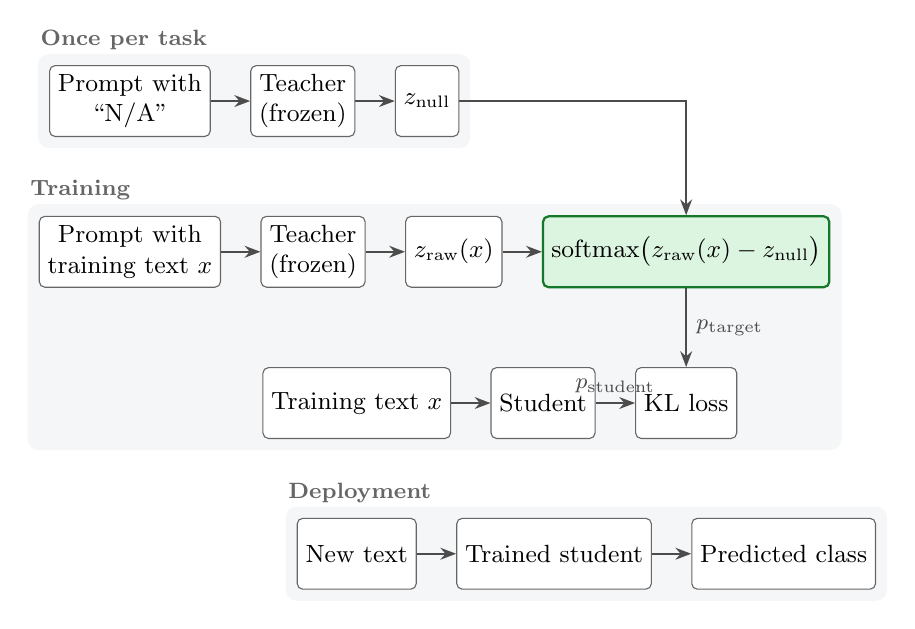
\begin{tikzpicture}[
  node distance=4mm and 5mm,
  box/.style={draw=black!60, rounded corners=2pt, align=center, font=\small, minimum height=9mm, inner sep=3pt, fill=white},
  key/.style={box, draw=textgreen, fill=cellgreen, thick},
  arr/.style={-{Stealth[length=2mm]}, thick, black!70},
  lane/.style={font=\footnotesize\bfseries, text=black!60, anchor=west}]
  % Row 1: null probe
  \node[box] (null) {Prompt with\\``N/A''};
  \node[box, right=of null] (t1) {Teacher\\(frozen)};
  \node[box, right=of t1] (zn) {$z_{\text{null}}$};
  % Row 2: targets
  \node[box, below=10mm of null] (x) {Prompt with\\training text $x$};
  \node[box, right=of x] (t2) {Teacher\\(frozen)};
  \node[box, right=of t2] (zr) {$z_{\text{raw}}(x)$};
  \node[key, right=of zr] (sub) {$\text{softmax}\big(z_{\text{raw}}(x) - z_{\text{null}}\big)$};
  % Row 3: student
  \node[box, below=10mm of sub] (kl) {KL loss};
  \node[box, left=of kl] (stu) {Student};
  \node[box, left=of stu] (xs) {Training text $x$};
  % Row 4: deployment
  \node[box, below=10mm of xs] (new) {New text};
  \node[box, right=of new] (stu2) {Trained student};
  \node[box, right=of stu2] (cls) {Predicted class};
  \draw[arr] (null) -- (t1); \draw[arr] (t1) -- (zn);
  \draw[arr] (x) -- (t2); \draw[arr] (t2) -- (zr); \draw[arr] (zr) -- (sub);
  \draw[arr] (zn) -| (sub);
  \draw[arr] (sub) -- node[right, font=\footnotesize] {$p_{\text{target}}$} (kl);
  \draw[arr] (xs) -- (stu); \draw[arr] (stu) -- node[above, font=\footnotesize] {$p_{\text{student}}$} (kl);
  \draw[arr] (new) -- (stu2); \draw[arr] (stu2) -- (cls);
  \begin{scope}[on background layer]
    \node[fill=lanegray, rounded corners, fit=(null)(zn), inner sep=4pt, label={[lane, anchor=south west, inner sep=1pt]north west:Once per task}] (l1) {};
    \node[fill=lanegray, rounded corners, fit=(x)(sub)(kl)(xs), inner sep=4pt, label={[lane, anchor=south west, inner sep=1pt]north west:Training}] {};
    \node[fill=lanegray, rounded corners, fit=(new)(cls), inner sep=4pt, label={[lane, anchor=south west, inner sep=1pt]north west:Deployment}] {};
  \end{scope}
\end{tikzpicture}}
\caption{Overview of Null Calibrated KD. We subtract the teacher's scores on ``N/A'' from its scores on every training text. Only the student runs at deployment.}
\label{fig:pipeline}
\end{figure}

First, we need to extract the teacher model's bias without probing it with an actual input.
For that, we pass it a null string, \texttt{"N/A"}, using the exact same classification prompt as for normal inference \& knowledge distillation \citep{zhao2021calibrate}.
The prompt lists each class next to an option letter (A, B, C and so on), as Figure~\ref{fig:prompt} and Appendix~\ref{app:prompts} show.
We read the teacher's logit for each letter, which is the unnormalised score the model gives to that token.

\begin{figure}[t]
\centering
\fbox{\parbox{0.94\columnwidth}{\small\ttfamily
Classify the news article into one of five categories:\\
A: Tech\\ B: Business\\ C: Sport\\ D: Entertainment\\ E: Politics\\[4pt]
Text: \textrm{\textit{input text, or} N/A \textit{for the null probe}}\\
Respond with ONLY the single letter corresponding to the correct category.\\
Answer:}}
\caption{Teacher prompt for BBC News. The null probe uses the same prompt with ``N/A'' as the text.}
\label{fig:prompt}
\end{figure}

Because there is no real input to classify, we start with the assumption that whatever the teacher outputs here is its baseline bias.
We extract these unnormalised logit values for all the candidate classes and call this the `Null' vector.All these effects mix in the teacher's output, and there is no single way to separate each one.
The null probe aims to measure their combined effect for one fixed prompt and one fixed option order.
As such, by subtracting the null logits, we aim to remove the combined prior bias before the student can learn it.

\begin{equation}
z_{\text{null}} = \text{Teacher}(\text{``N/A''})
\end{equation}

Once we have captured this, we run the teacher model over our unlabelled training set and extract the raw logit vector $z_{\text{raw}}$ for each example.
Instead of directly plugging them into the loss function, we first perform a simple logit subtraction to get the debiased target.
\begin{equation}
\tilde{z} = z_{\text{raw}} - z_{\text{null}}
\end{equation}

This is a constant-time, $O(1)$ operation per example, which does not impact the compute required or the time taken.
After this, we apply the softmax function, which turns these logits into actual probabilities.
\begin{equation}
p_{\text{target},k} = \text{softmax}(\tilde{z})_k = \frac{\exp(\tilde{z}_k)}{\sum_{j} \exp(\tilde{z}_j)}
\end{equation}

Now we can train our compact student model (RoBERTa-base) using forward Kullback-Leibler (KL) divergence as our loss function.
KL divergence measures how far one probability distribution is from another \citep{kullback1951information}.
It helps in training the student model by bringing the student's predicted probability distribution as close as possible to the teacher's debiased target distribution.
\begin{equation}
\mathcal{L} = D_{\text{KL}}(p_{\text{target}} \parallel p_{\text{student}})
\end{equation}

\section{Experimental Setup}

\subsection{Datasets}

To test this method, we ran the pipeline on 6 different multi-class classification tasks.
The datasets used are publicly available, and Table~\ref{tab:datasets} lists them.
We have used a fixed-size subset from each dataset using stratified sampling to preserve natural class skew.
Stratified sampling keeps the share of each class equal to its share in the full dataset.
We have selected a standardised split of 75:25 (1,200 training and 400 test) for training and testing.

\begin{table}[t]
\centering
\small
\resizebox{\columnwidth}{!}{
\begin{tabular}{llc}
\toprule
\textbf{Dataset} & \textbf{Domain} & $K$ \\
\midrule
Student Questions\footnotemark & Science subjects & 4 \\
TREC-6 \citep{li2002learning} & Question types & 6 \\
App Reviews \citep{grano2017android} & Review ratings & 5 \\
Twitter Emotion \citep{saravia2018carer} & Emotions & 6 \\
TweetEval \citep{barbieri2020tweeteval} & Emotions & 4 \\
BBC News \citep{greene2006practical} & News topics & 5 \\
\bottomrule
\end{tabular}
}
\caption{Datasets and their number of classes $K$. Each dataset contributes 1,200 training and 400 test examples. Table~\ref{tab:prompts} lists the classes.}
\label{tab:datasets}
\end{table}
\footnotetext{\url{https://huggingface.co/datasets/SetFit/student-question-categories}}

\subsection{Models}

We use the following models.
\begin{itemize}
    \item \textbf{Gemma-3-4B-IT} \citep{gemma2025gemma3}: We used this 4-billion-parameter instruction-tuned causal LLM as the teacher model, kept completely frozen in 16-bit precision.
    \item \textbf{RoBERTa-base} \citep{liu2019roberta}: This masked encoder model (125 million parameters) works as a lightweight student model. It consumes less memory and runs faster.
\end{itemize}
Table~\ref{tab:hparams} lists the student's training settings, which are the same for all methods.

\begin{table}[t]
\centering
\small
\resizebox{\columnwidth}{!}{
\begin{tabular}{ll}
\toprule
\textbf{Setting} & \textbf{Value} \\
\midrule
Optimizer & AdamW, weight decay 0.01 \\
Learning rate & $2 \times 10^{-5}$ \\
Schedule & Linear, 10\% warmup \\
Batch size & 16 \\
Epochs & 3 \\
Maximum sequence length & 256 tokens \\
Gradient clipping & 1.0 \\
Random seed & 42 \\
\bottomrule
\end{tabular}
}
\caption{Student training settings, shared by all methods.}
\label{tab:hparams}
\end{table}

\subsection{Baselines}

We compare null-calibrated KD against a few existing methods to see if we actually see any improvements.
\begin{itemize}
    \item \textbf{Teacher Zero-Shot:} The teacher LLM evaluated both with and without null calibration.
    \item \textbf{Standard Knowledge Distillation:} Distillation using the teacher's soft probabilities with forward KL divergence, but without calibration.
    \item \textbf{Batch-Calibrated KD:} The teacher's predictions are averaged across the entire training dataset to estimate class priors. Then we subtract them before computing distillation targets \citep{zhou2024batch}.
    \item \textbf{Null Calibrated KD:} Our method as explained above.
\end{itemize}

\begin{table*}[t]
\centering
\small
\resizebox{\textwidth}{!}{
\begin{tabular}{llcccccc}
\toprule
 & \textbf{Method} & \textbf{Student Questions} & \textbf{TREC-6} & \textbf{App Reviews} & \textbf{Twitter Emotion} & \textbf{TweetEval Emotion} & \textbf{BBC News} \\
 & & ($K=4$) & ($K=6$) & ($K=5$) & ($K=6$) & ($K=4$) & ($K=5$) \\
\midrule
Teacher & Zero-shot, raw & 28.13 (33.75) & \worst{50.15 (52.25)} & \worst{29.69 (48.25)} & 39.80 (53.00) & 45.78 (57.25) & \worst{54.81 (56.00)} \\
(Gemma-3-4B-IT) & Zero-shot, null-calibrated & 29.08 (33.75) & 52.90 (54.25) & 32.46 (49.25) & \best{40.35 (52.00)} & \best{56.05 (65.00)} & 64.04 (63.25) \\
\midrule
Student & Standard KD & \worst{22.86 (32.25)} & 62.28 (59.75) & 30.25 (51.75) & \worst{29.78 (50.50)} & \worst{34.16 (54.25)} & 55.56 (58.50) \\
(RoBERTa-base) & Batch-Calibrated KD & 23.19 (32.00) & 63.29 (61.00) & 32.04 (52.25) & 31.13 (50.00) & 38.85 (56.50) & 57.13 (60.25) \\
 & Null Calibrated KD (ours) & \best{37.10 (39.25)} & \best{64.71 (61.75)} & \best{33.24 (53.25)} & 34.46 (50.75) & 55.48 (66.50) & \best{71.40 (70.50)} \\
\bottomrule
\end{tabular}
}
\caption{Macro-F1 with accuracy in parentheses, both in \%, on the 400 test examples of each dataset. Green marks the highest and red the lowest Macro-F1 in each column.}
\label{tab:main_results}
\end{table*}

\begin{figure*}[t]
\centering
\resultfig{generated/fig_main_f1_accuracy.pdf}{0.36}
\caption{Macro-F1 and accuracy of the raw teacher and three distillation methods on all six datasets.}
\label{fig:main_results}
\end{figure*}
\begin{figure*}[t]
\centering
\resultfig{generated/fig_class_distributions.pdf}{0.30}
\caption{Number of test predictions per class on three datasets. The dotted line shows the true number of test examples in each class.}
\label{fig:class_dist}
\end{figure*}

\subsection{Metrics}

For capturing this quantitatively, we use \textbf{Macro-F1}.
F1 combines precision and recall, and Macro-F1 averages the F1 score of every class.
This helps us to measure fairly across the minority and dominant classes alike.
It gives equal weight to all K classes, so a model cannot score better by simply over predicting the majority class.
We also report overall \textbf{Accuracy} as a secondary metric.

\section{Results}

We ran our pipeline across all these datasets and captured the required metrics.
We answer three research questions (RQs).
\begin{enumerate}
    \item[\textbf{RQ1.}] Does null calibration improve the student's Macro-F1 and Accuracy?
    \item[\textbf{RQ2.}] Does null calibration reduce class collapse?
    \item[\textbf{RQ3.}] Can null calibration over-correct?
\end{enumerate}




\subsection{RQ1: Macro-F1 and Accuracy}

Table~\ref{tab:main_results} captures Macro-F1 and Accuracy across all 6 datasets and all different methods, and Figure~\ref{fig:main_results} plots them.
Null calibrated KD improves Macro-F1 over standard KD on \WinsStd{} out of 6 datasets.
Macro-F1 increases by \AvgGainStd{} pp on average, with the largest gain on \MaxGainStdData{} (\MaxGainStd{} pp).
Accuracy increases by \AvgAccGainStd{} pp on average.
Null calibrated KD also beats batch-calibrated KD on \WinsBatch{} out of 6 datasets.
The student even beats the raw teacher on \WinsTeacher{} out of 6 datasets.

\subsection{RQ2: Class Collapse}

\begin{table}[t]
\centering
\small
\resizebox{\columnwidth}{!}{
\begin{tabular}{llrrrrr}
\toprule
\textbf{Dataset} & \textbf{Class} & \textbf{True} & \textbf{Teacher} & \textbf{Std.} & \textbf{Batch} & \textbf{Null} \\
\midrule
Student Questions & Chemistry & 43 & 12 & \textbf{0} & \textbf{0} & 18 \\
App Reviews & 4 Stars & 55 & 22 & \textbf{0} & 16 & 30 \\
Twitter Emotion & Fear & 48 & 19 & \textbf{0} & \textbf{0} & 5 \\
Twitter Emotion & Surprise & 14 & \textbf{0} & \textbf{0} & \textbf{0} & \textbf{0} \\
TweetEval Emotion & Optimism & 36 & 10 & \textbf{0} & 1 & 6 \\
BBC News & Politics & 75 & 15 & \textbf{0} & 8 & 51 \\
\bottomrule
\end{tabular}
}
\caption{Number of test predictions for every class that at least one distillation method never predicts. True is the number of test examples in the class. Std., Batch and Null denote standard, Batch-Calibrated and Null Calibrated KD. Bold marks zero predictions.}
\label{tab:collapse}
\end{table}


Apart from improving Macro-F1 and Accuracy, null calibration reduces the collapse of certain classes and the over-boosting of others.
Table~\ref{tab:collapse} and Figure~\ref{fig:class_dist} show this.
We can see that standard KD completely collapses minority classes across multiple tasks.
It makes 0 predictions for \textit{Politics} on BBC News, \textit{Optimism} on TweetEval, and \textit{Chemistry} on Student Questions.
Null-calibrated KD actively helps us avoid the same, and it also recovers \textit{Fear} on Twitter Emotion.
\textit{Surprise} on Twitter Emotion stays at 0 predictions for every method, including the teacher.
Null calibration also reduces overly boosted classes, such as \textit{Business} on BBC News and \textit{Anger} on TweetEval.

\subsection{RQ3: Over-Correction}
\label{sec:overcorrection}

The null probe can also over-correct, as Table~\ref{tab:collapse} shows.
\OverCorrectionText{}
A very strong null bias can therefore push a class below what the data supports.
The Student Questions case shows that this combined estimate can sometimes be too strong.


\section{Conclusion}

LLM teachers have built-in prompt and token biases that can affect knowledge distillation using soft targets.
It causes smaller student models to learn the bias, and as a result, they sometimes completely collapse on minority classes.
A single offline probe with a blank prompt (\texttt{N/A}) can capture this bias.
We subtract these null logits inside the distillation loss function before the student can learn from it.
Students show better performance, sometimes even better than the teacher.
Macro-F1 increases by an average of \textbf{\AvgGainStd{}\,pp} on the tested datasets.
This helps reduce class collapse and overboosting.
The method needs only one extra teacher query and no human intervention.
However, a very strong null bias can lead to over-correction, as on Student Questions.

\section*{Limitations}

Even though this method works, there are a few limitations to it.
\begin{enumerate}
    \item If the teacher itself is very bad (near random), then this method cannot manufacture knowledge which did not exist.
    \item We have limited the scope to multi-class classification tasks. For sequence generation tasks, our method is not applicable.
    \item In certain cases where the teacher itself has an almost flat distribution (carries low bias), we might see minimal or even negative impact. As such, developers' discretion is advised.
    \item When the teacher's null bias is very strong, subtracting it can remove a class entirely (Section~\ref{sec:overcorrection}).
    \item On simple, uniformly balanced tasks or binary tasks, standard KD may already be sufficient.
    \item We use a single teacher, a single student and a single random seed.
\end{enumerate}

\section*{Acknowledgments}

We thank Prof.Dhruv Kumar (Faculty/Advisor) and Aniket Upadhyay (Mentor) for their valuable feedbacks and suggestions.

\bibliography{references}
\bibliographystyle{acl_natbib}

\appendix

\section{Teacher Prompts}
\label{app:prompts}

Table~\ref{tab:prompts} lists the task description that opens the prompt for each dataset.
The prompt then lists the classes next to the letters A, B, C and so on, in the order of the table.
The prompt then continues with the input text and the instruction shown in Figure~\ref{fig:prompt}.

\begin{table}[h]
\centering
\small
\begin{tabular}{>{\raggedright\arraybackslash}p{0.24\columnwidth}>{\raggedright\arraybackslash}p{0.64\columnwidth}}
\toprule
\textbf{Dataset} & \textbf{Task description} \newline \textit{Classes, in option order A, B, C, \ldots} \\
\midrule
Student Questions & Classify the academic question into the correct subject: \newline \textit{Biology, Physics, Maths, Chemistry} \\[3pt]
TREC-6 & Classify the question into one of six question types: \newline \textit{Abbreviation, Entity, Description, Human, Location, Numeric} \\[3pt]
App Reviews & Classify the customer app review into one of five star ratings: \newline \textit{1 Star, 2 Stars, 3 Stars, 4 Stars, 5 Stars} \\[3pt]
Twitter Emotion & Classify the tweet into one of six emotions: \newline \textit{Sadness, Joy, Love, Anger, Fear, Surprise} \\[3pt]
TweetEval & Classify the tweet into one of four emotions: \newline \textit{Anger, Joy, Optimism, Sadness} \\[3pt]
BBC News & Classify the news article into one of five categories: \newline \textit{Tech, Business, Sport, Entertainment, Politics} \\[3pt]
\bottomrule
\end{tabular}
\caption{Task descriptions and classes used in the teacher prompts.}
\label{tab:prompts}
\end{table}

\subsection{Full Prompt Template}
\label{app:prompt_template}

Every teacher call uses the same template, shown in Figure~\ref{fig:app_prompt_template}.
\texttt{\{task\_desc\}} is the task description of Table~\ref{tab:prompts} followed by one line per class, in the form \texttt{A: Biology}.
\texttt{\{text\}} is the input text with surrounding whitespace removed, cut to its first 600 characters.
The full prompt is then cut to 256 tokens from the left, so the instruction at the end is always kept.
For the null probe, \texttt{\{text\}} is the string \texttt{N/A}, and the probe is run once per task.

\begin{figure}[h]
\centering
\fbox{\parbox{0.94\columnwidth}{\small\ttfamily
\{task\_desc\}\\
A: \{class 1\}\\ B: \{class 2\}\\ \ldots\\[4pt]
Text: \{text\}\\
Respond with ONLY the single letter corresponding to the correct category.\\
Answer:}}
\caption{Prompt template shared by all datasets. No chat template or system prompt is added.}
\label{fig:app_prompt_template}
\end{figure}

We read the logits of the teacher at the last position of the prompt.
For each class, we keep the logit of the token for its option letter (\texttt{A}, \texttt{B}, \ldots) and drop every other token.
These $K$ numbers form $z_{\text{raw}}(x)$ for a training text $x$, and $z_{\text{null}}$ for the null probe.
The teacher's zero-shot prediction is the class with the highest of these $K$ logits.

Below is the full null probe for Student Questions, exactly as the teacher sees it.

\begin{figure}[h]
\centering
\fbox{\parbox{0.94\columnwidth}{\small\ttfamily
Classify the academic question into the correct subject:\\
A: Biology\\ B: Physics\\ C: Maths\\ D: Chemistry\\[4pt]
Text: N/A\\
Respond with ONLY the single letter corresponding to the correct category.\\
Answer:}}
\caption{Null probe prompt for Student Questions.}
\label{fig:app_null_prompt}
\end{figure}

\paragraph{Prompts in the ablations.}
The cross-family setting of Ablation~1 uses Qwen3-4B as the teacher with the same template.
The causal LoRA students of Ablation~1 also receive the same template, and they are trained to match the target distribution over the option letters.
Ablation~4 rotates the order of the classes in the option list, so that every class appears once under every letter.
For a task with four classes, the four orders are $(1,2,3,4)$, $(2,3,4,1)$, $(3,4,1,2)$ and $(4,1,2,3)$.
The probabilities of each order are mapped back to the original class order and averaged.

\FloatBarrier
\section{Teacher Bias Measured by the Null Probe}
\label{app:null_logits}

Table~\ref{tab:app_null_logits} and Figure~\ref{fig:app_null_logits} show the null vector $z_{\text{null}}$ of Gemma-3-4B-IT for each dataset.
On all six datasets the teacher gives the highest null logit to option \texttt{A}, which is the first class in the list.
This matches the token and position biases discussed in the main text.
On BBC News, option \texttt{B} (Business) is almost as high as \texttt{A}, which fits the over-prediction of Business by the raw teacher and standard KD.

\begin{table*}[t]
\centering
\small
\resizebox{\textwidth}{!}{
\begin{tabular}{l>{\raggedright\arraybackslash}p{0.62\textwidth}lc}
\toprule
\textbf{Dataset} & \textbf{Null logits $z_{\text{null}}$ (class~logit)} & \textbf{Favoured class} & \textbf{Gap (max$-$min)} \\
\midrule
Student Questions & Biology~16.12, Physics~10.00, Maths~10.19, Chemistry~9.06 & Biology & 7.06 \\
TREC-6 & Abbreviation~16.00, Entity~12.19, Description~14.06, Human~10.94, Location~11.25, Numeric~11.19 & Abbreviation & 5.06 \\
App Reviews & 1 Star~15.06, 2 Stars~10.19, 3 Stars~10.50, 4 Stars~8.25, 5 Stars~7.38 & 1 Star & 7.69 \\
Twitter Emotion & Sadness~16.12, Joy~12.88, Love~12.62, Anger~10.56, Fear~10.25, Surprise~10.06 & Sadness & 6.06 \\
TweetEval Emotion & Anger~15.56, Joy~9.69, Optimism~10.62, Sadness~9.44 & Anger & 6.12 \\
BBC News & Tech~16.62, Business~16.50, Sport~12.56, Entertainment~10.94, Politics~10.44 & Tech & 6.19 \\
\bottomrule
\end{tabular}
}
\caption{Gemma-3-4B-IT logits for each option letter when the prompt contains ``N/A'' instead of a real input. The favoured class is the one the teacher prefers before it reads any text. A larger gap means a stronger prior bias.}
\label{tab:app_null_logits}
\end{table*}


\begin{figure*}[t]
\centering
\resultfig{generated/fig_app_null_logits.pdf}{0.45}
\caption{Null logits of Gemma-3-4B-IT, centred on their mean for each dataset. Red bars are classes the teacher prefers before reading any input, blue bars are classes it disfavours.}
\label{fig:app_null_logits}
\end{figure*}

\FloatBarrier
\section{Additional Results}
\label{app:additional}

This section gives the full per-class results of the main experiment (Table~\ref{tab:main_results}).
Table~\ref{tab:app_per_class_f1} lists the F1 score of every class.
Table~\ref{tab:app_counts} and Figure~\ref{fig:app_class_dist_all} list how often each method predicts each class, for all six datasets.
Table~\ref{tab:collapse} in the main text is a subset of Table~\ref{tab:app_counts}.

\begin{table}[!ht]
\centering
\scriptsize
\setlength{\tabcolsep}{4pt}
\resizebox{\ifdim\width>\columnwidth\columnwidth\else\width\fi}{!}{%
\begin{tabular}{@{}lrrrrrrr@{}}
\toprule
\textbf{Method} & \multicolumn{6}{c}{\textbf{F1 of each class}} & \textbf{Worst} \\
\midrule
\textit{Student Questions} & \textit{Biology} & \textit{Physics} & \textit{Maths} & \textit{Chemistry} & & & \textit{Worst} \\
Teacher, raw & \textbf{17.43} & 17.14 & 61.70 & 10.91 & & & 10.91 \\
Teacher, null-cal. & 2.80 & \textbf{21.29} & 59.06 & 31.25 & & & 2.80 \\
Standard KD & 10.33 & 11.62 & 66.67 & \worst{0.00} & & & 0.00 \\
Batch-Cal. KD & 10.28 & 12.96 & \textbf{68.24} & \worst{0.00} & & & 0.00 \\
Null-Cal. KD (ours) & 1.47 & 16.54 & 59.35 & \textbf{45.90} & & & 1.47 \\
\midrule
\textit{TREC-6} & \textit{Abbr.} & \textit{Entity} & \textit{Desc.} & \textit{Human} & \textit{Location} & \textit{Numeric} & \textit{Worst} \\
Teacher, raw & 38.46 & 10.94 & 55.28 & 57.83 & 70.59 & 67.83 & 10.94 \\
Teacher, null-cal. & 43.48 & 19.40 & 58.67 & 54.14 & 72.73 & 68.97 & 19.40 \\
Standard KD & 76.92 & 22.22 & 59.35 & \textbf{65.14} & 75.44 & 74.60 & 22.22 \\
Batch-Cal. KD & 75.00 & 27.07 & 61.21 & 64.41 & 76.11 & \textbf{75.97} & 27.07 \\
Null-Cal. KD (ours) & \textbf{83.33} & \textbf{28.12} & \textbf{65.49} & 62.18 & \textbf{79.67} & 69.49 & 28.12 \\
\midrule
\textit{App Reviews} & \textit{1 Star} & \textit{2 Stars} & \textit{3 Stars} & \textit{4 Stars} & \textit{5 Stars} & & \textit{Worst} \\
Teacher, raw & 55.26 & 10.96 & 5.26 & 10.39 & 69.94 & & 5.26 \\
Teacher, null-cal. & \textbf{65.17} & 8.51 & 5.88 & \textbf{16.51} & 70.66 & & 5.88 \\
Standard KD & 57.27 & \textbf{12.31} & 9.52 & \worst{0.00} & 76.60 & & 0.00 \\
Batch-Cal. KD & 59.05 & 8.11 & 7.89 & 8.45 & 74.80 & & 7.89 \\
Null-Cal. KD (ours) & 63.16 & 9.80 & \textbf{10.34} & 7.06 & \textbf{77.60} & & 7.06 \\
\midrule
\textit{Twitter Emotion} & \textit{Sadness} & \textit{Joy} & \textit{Love} & \textit{Anger} & \textit{Fear} & \textit{Surprise} & \textit{Worst} \\
Teacher, raw & \textbf{62.58} & 56.04 & 30.77 & \textbf{44.63} & 44.78 & \worst{0.00} & 0.00 \\
Teacher, null-cal. & 61.28 & 55.77 & \textbf{35.29} & 42.55 & \textbf{47.22} & \worst{0.00} & 0.00 \\
Standard KD & 58.47 & \textbf{66.38} & 28.00 & 25.81 & \worst{0.00} & \worst{0.00} & 0.00 \\
Batch-Cal. KD & 57.65 & 63.11 & 25.00 & 41.03 & \worst{0.00} & \worst{0.00} & 0.00 \\
Null-Cal. KD (ours) & 57.89 & 64.32 & 32.14 & 41.10 & 11.32 & \worst{0.00} & 0.00 \\
\midrule
\textit{TweetEval Emotion} & \textit{Anger} & \textit{Joy} & \textit{Optimism} & \textit{Sadness} & & & \textit{Worst} \\
Teacher, raw & 67.07 & 62.77 & 34.78 & 18.49 & & & 18.49 \\
Teacher, null-cal. & 72.93 & 74.07 & \textbf{38.30} & 38.89 & & & 38.30 \\
Standard KD & 65.49 & 65.73 & \worst{0.00} & 5.41 & & & 0.00 \\
Batch-Cal. KD & 66.53 & 66.21 & 5.41 & 17.24 & & & 5.41 \\
Null-Cal. KD (ours) & \textbf{73.42} & \textbf{74.68} & 23.81 & \textbf{50.00} & & & 23.81 \\
\midrule
\textit{BBC News} & \textit{Tech} & \textit{Business} & \textit{Sport} & \textit{Entert.} & \textit{Politics} & & \textit{Worst} \\
Teacher, raw & 51.85 & 51.98 & 78.15 & 55.67 & 26.67 & & 26.67 \\
Teacher, null-cal. & 51.92 & 56.60 & 80.52 & 64.76 & 60.50 & & 51.92 \\
Standard KD & 50.00 & 51.11 & 84.28 & 74.55 & \worst{0.00} & & 0.00 \\
Batch-Cal. KD & \textbf{72.57} & 55.26 & 86.42 & 73.39 & 19.28 & & 19.28 \\
Null-Cal. KD (ours) & 61.54 & \textbf{65.71} & \textbf{90.48} & \textbf{86.89} & \textbf{76.19} & & 61.54 \\
\bottomrule
\end{tabular}}
\caption{Per-class F1 (\%) on the 400 test examples of each dataset. Bold marks the best method for each class, red marks a class with F1 of 0. Worst is the lowest per-class F1 of the row.}
\label{tab:app_per_class_f1}
\end{table}


\begin{figure*}[t]
\centering
\resultfig{generated/fig_app_class_dist_all.pdf}{0.55}
\caption{Number of test predictions per class on all six datasets. The dotted line shows the true number of test examples in each class.}
\label{fig:app_class_dist_all}
\end{figure*}

\begin{table}[!ht]
\centering
\scriptsize
\setlength{\tabcolsep}{4pt}
\resizebox{\ifdim\width>\columnwidth\columnwidth\else\width\fi}{!}{%
\begin{tabular}{@{}lrrrrrr@{}}
\toprule
\textbf{Class} & \textbf{True} & \textbf{Teach.} & \textbf{T.+Null} & \textbf{Std.} & \textbf{Batch} & \textbf{Null} \\
\midrule
\multicolumn{7}{@{}l}{\textit{Student Questions}} \\
\quad Biology & 126 & 100 & 19 & 90 & 94 & \textbf{0} \\
\quad Physics & 123 & 106 & 119 & 121 & 120 & 139 \\
\quad Maths & 108 & 183 & 197 & 189 & 179 & 208 \\
\quad Chemistry & 43 & 11 & 65 & \textbf{0} & 7 & 53 \\
\multicolumn{7}{@{}l}{\textit{TREC-6}} \\
\quad Abbreviation & 7 & 19 & 16 & 6 & 9 & 5 \\
\quad Entity & 91 & 37 & 43 & 35 & 42 & 37 \\
\quad Description & 94 & 152 & 131 & 152 & 138 & 132 \\
\quad Human & 76 & 90 & 105 & 99 & 101 & 117 \\
\quad Location & 62 & 57 & 59 & 52 & 51 & 61 \\
\quad Numeric & 70 & 45 & 46 & 56 & 59 & 48 \\
\multicolumn{7}{@{}l}{\textit{App Reviews}} \\
\quad 1 Star & 68 & 164 & 116 & 157 & 145 & 110 \\
\quad 2 Stars & 24 & 48 & 70 & 33 & 41 & 70 \\
\quad 3 Stars & 36 & 37 & 29 & 60 & 50 & 18 \\
\quad 4 Stars & 55 & 22 & 48 & 1 & 15 & 37 \\
\quad 5 Stars & 217 & 129 & 137 & 149 & 149 & 165 \\
\multicolumn{7}{@{}l}{\textit{Twitter Emotion}} \\
\quad Sadness & 117 & 209 & 180 & 249 & 223 & 187 \\
\quad Joy & 135 & 72 & 73 & 94 & 90 & 92 \\
\quad Love & 32 & 33 & 36 & 18 & 24 & 24 \\
\quad Anger & 54 & 67 & 87 & 39 & 63 & 92 \\
\quad Fear & 48 & 19 & 24 & \textbf{0} & \textbf{0} & 5 \\
\quad Surprise & 14 & \textbf{0} & \textbf{0} & \textbf{0} & \textbf{0} & \textbf{0} \\
\multicolumn{7}{@{}l}{\textit{TweetEval Emotion}} \\
\quad Anger & 167 & 331 & 280 & 343 & 335 & 277 \\
\quad Joy & 91 & 46 & 71 & 52 & 54 & 67 \\
\quad Optimism & 36 & 10 & 11 & \textbf{0} & 1 & 6 \\
\quad Sadness & 106 & 13 & 38 & 5 & 10 & 50 \\
\multicolumn{7}{@{}l}{\textit{BBC News}} \\
\quad Tech & 72 & 54 & 46 & 41 & 42 & 41 \\
\quad Business & 92 & 247 & 217 & 256 & 249 & 209 \\
\quad Sport & 92 & 58 & 64 & 63 & 66 & 71 \\
\quad Entertainment & 69 & 27 & 37 & 40 & 43 & 54 \\
\quad Politics & 75 & 14 & 36 & \textbf{0} & \textbf{0} & 25 \\
\bottomrule
\end{tabular}}
\caption{Number of test predictions per class for every dataset and method. True is the number of test examples in the class. Teach.\ and T.+Null are the raw and null-calibrated teacher; Std., Batch and Null are the three distillation methods. Bold marks a class that is never predicted.}
\label{tab:app_counts}
\end{table}


\FloatBarrier
\section{Ablation Studies}
\label{app:ablations}

We run five ablations to test whether the gains of null calibration hold beyond the main setting.
Unless stated otherwise, every ablation uses the datasets, splits, teacher logits and student settings of the main experiment (Table~\ref{tab:hparams}).
Each ablation is a separate training run, so numbers for the same method can differ slightly from Table~\ref{tab:main_results}.

\subsection{Ablation 1: Other Architectures}
\label{app:abl_arch}

We test three other teacher and student pairs, each on one dataset.
\begin{itemize}
    \item \textbf{Same-size:} Gemma-3-4B-IT distils into Qwen3-4B, a student of the same size, on BBC News.
    \item \textbf{Cross-family:} Qwen3-4B is the teacher and RoBERTa-base the student, on TweetEval Emotion. The null probe is run on Qwen3-4B.
    \item \textbf{Small SLM:} Gemma-3-4B-IT distils into Qwen2.5-0.5B, a small causal LM, on TREC-6.
\end{itemize}
The causal students are fine-tuned with LoRA (rank 16, $\alpha = 32$, dropout 0.05) for 2 epochs with learning rate $5 \times 10^{-5}$.
Table~\ref{tab:app_ablation1} shows that null calibration improves Macro-F1 in all three settings.
The gain is small in the cross-family setting, where the Qwen3-4B teacher is already strong on TweetEval Emotion, and accuracy drops by 2.25 pp.

\begin{table*}[t]
\centering
\small
\resizebox{\textwidth}{!}{
\begin{tabular}{llllccc}
\toprule
\textbf{Setting} & \textbf{Teacher} & \textbf{Student} & \textbf{Dataset} & \textbf{Standard KD} & \textbf{Null-Cal. KD (ours)} & \textbf{$\Delta$ F1 (pp)} \\
\midrule
Same-size & Gemma-3-4B-IT & Qwen3-4B (LoRA) & BBC News & 57.14 (60.50) & \textbf{65.17} (67.25) & \textcolor{textgreen}{+8.02} \\
Cross-family & Qwen3-4B & RoBERTa-base & TweetEval Emotion & 69.29 (77.00) & \textbf{69.85} (74.75) & \textcolor{textgreen}{+0.56} \\
Small SLM & Gemma-3-4B-IT & Qwen2.5-0.5B (LoRA) & TREC-6 & 19.94 (32.75) & \textbf{26.93} (39.75) & \textcolor{textgreen}{+6.99} \\
\bottomrule
\end{tabular}
}
\caption{Ablation 1: other teacher and student architectures. Macro-F1 with accuracy in parentheses, both in \%. The LoRA students are causal LMs trained to predict the option letter.}
\label{tab:app_ablation1}
\end{table*}


\subsection{Ablation 2: Multi-Task Distillation}
\label{app:abl_multitask}

Here one RoBERTa-base encoder learns several tasks at once, with a separate linear classification head for each task.
Each task keeps its own null vector, which is subtracted from the logits of that task only.
Table~\ref{tab:app_ablation2} reports the average Macro-F1 over the tasks of each combination, and Table~\ref{tab:app_ablation2_per_task} and Figure~\ref{fig:app_multitask} report each task.
Null calibration improves the average Macro-F1 in all five combinations, by 3.93 to 15.63 pp.
It also improves Macro-F1 on every task of every combination.

\begin{table}[!ht]
\centering
\footnotesize
\setlength{\tabcolsep}{4pt}
\resizebox{\ifdim\width>\columnwidth\columnwidth\else\width\fi}{!}{%
\begin{tabular}{@{}c>{\raggedright\arraybackslash}p{0.42\columnwidth}ccc@{}}
\toprule
\textbf{\#} & \textbf{Tasks sharing one student} & \textbf{Std. KD} & \textbf{Null-Cal.} & \textbf{$\Delta$ F1} \\
\midrule
1 & TweetEval Emotion + BBC News & 51.04 & \textbf{66.32} & \textcolor{textgreen}{+15.28} \\
2 & BBC News + TREC-6 & 60.32 & \textbf{67.17} & \textcolor{textgreen}{+6.85} \\
3 & Twitter Emotion + TREC-6 & 48.96 & \textbf{52.89} & \textcolor{textgreen}{+3.93} \\
4 & TweetEval Emotion + BBC News + TREC-6 & 51.52 & \textbf{64.88} & \textcolor{textgreen}{+13.36} \\
5 & TweetEval Emotion + BBC News + App Reviews + Twitter Emotion + TREC-6 & 45.57 & \textbf{52.78} & \textcolor{textgreen}{+7.21} \\
\bottomrule
\end{tabular}}
\caption{Ablation 2: multi-task distillation into one RoBERTa-base encoder with a separate classification head per task. Macro-F1 (\%) averaged over the tasks of each combination.}
\label{tab:app_ablation2}
\end{table}

\begin{table}[!ht]
\centering
\scriptsize
\setlength{\tabcolsep}{4pt}
\resizebox{\ifdim\width>\columnwidth\columnwidth\else\width\fi}{!}{%
\begin{tabular}{@{}clccc@{}}
\toprule
\textbf{\#} & \textbf{Task} & \textbf{Std. KD} & \textbf{Null-Cal.} & \textbf{$\Delta$ F1} \\
\midrule
1 & TweetEval Emotion & 44.22 (58.00) & 60.52 (69.50) & \textcolor{textgreen}{+16.30} \\
 & BBC News & 57.86 (60.50) & 72.12 (70.75) & \textcolor{textgreen}{+14.26} \\
\midrule
2 & BBC News & 60.42 (62.50) & 72.81 (71.50) & \textcolor{textgreen}{+12.39} \\
 & TREC-6 & 60.22 (58.25) & 61.53 (60.00) & \textcolor{textgreen}{+1.31} \\
\midrule
3 & Twitter Emotion & 38.62 (53.50) & 43.63 (56.75) & \textcolor{textgreen}{+5.01} \\
 & TREC-6 & 59.31 (57.75) & 62.15 (59.25) & \textcolor{textgreen}{+2.84} \\
\midrule
4 & TweetEval Emotion & 38.03 (55.50) & 59.39 (70.00) & \textcolor{textgreen}{+21.36} \\
 & BBC News & 59.24 (62.00) & 74.70 (73.25) & \textcolor{textgreen}{+15.46} \\
 & TREC-6 & 57.30 (55.50) & 60.55 (57.75) & \textcolor{textgreen}{+3.25} \\
\midrule
5 & TweetEval Emotion & 43.54 (57.25) & 56.77 (66.00) & \textcolor{textgreen}{+13.23} \\
 & BBC News & 57.14 (60.25) & 69.80 (69.25) & \textcolor{textgreen}{+12.65} \\
 & App Reviews & 31.24 (52.75) & 35.72 (55.50) & \textcolor{textgreen}{+4.48} \\
 & Twitter Emotion & 36.81 (52.25) & 40.90 (54.50) & \textcolor{textgreen}{+4.10} \\
 & TREC-6 & 59.12 (57.00) & 60.70 (57.00) & \textcolor{textgreen}{+1.58} \\
\bottomrule
\end{tabular}}
\caption{Ablation 2, per task: Macro-F1 with accuracy in parentheses, both in \%.}
\label{tab:app_ablation2_per_task}
\end{table}


\begin{figure*}[t]
\centering
\resultfig{generated/fig_app_multitask.pdf}{0.30}
\caption{Ablation 2: Macro-F1 of each task when several tasks share one student.}
\label{fig:app_multitask}
\end{figure*}

\subsection{Ablation 3: Hard Labels versus Soft Targets}
\label{app:abl_hard_soft}

A simpler way to use the teacher is to train on its top class only, as a hard pseudo-label, with cross-entropy loss.
Table~\ref{tab:app_ablation3} compares hard labels and soft targets, with and without null calibration, on BBC News and TweetEval Emotion.
Null calibration helps both kinds of target.
Null-calibrated soft targets give the best Macro-F1 and accuracy on both datasets.
Calibrated hard labels come second, which shows that the full calibrated distribution carries useful information beyond the top class.

\begin{table*}[t]
\centering
\small
\begin{tabular}{lllccc}
\toprule
\textbf{Dataset} & \textbf{Regime} & \textbf{Target} & \textbf{Loss} & \textbf{Macro-F1} & \textbf{Accuracy} \\
\midrule
BBC News & Raw hard labels & $\arg\max z_{\text{raw}}$ & Cross-entropy & 55.95 & 59.00 \\
 & Calibrated hard labels & $\arg\max (z_{\text{raw}} - z_{\text{null}})$ & Cross-entropy & 58.93 & 61.75 \\
 & Standard soft KD & $\text{softmax}(z_{\text{raw}})$ & KL & 55.02 & 58.00 \\
 & Null-Cal. soft KD (ours) & $\text{softmax}(z_{\text{raw}} - z_{\text{null}})$ & KL & \textbf{71.58} & 70.50 \\
\midrule
TweetEval Emotion & Raw hard labels & $\arg\max z_{\text{raw}}$ & Cross-entropy & 32.43 & 53.00 \\
 & Calibrated hard labels & $\arg\max (z_{\text{raw}} - z_{\text{null}})$ & Cross-entropy & 47.88 & 64.25 \\
 & Standard soft KD & $\text{softmax}(z_{\text{raw}})$ & KL & 34.16 & 54.25 \\
 & Null-Cal. soft KD (ours) & $\text{softmax}(z_{\text{raw}} - z_{\text{null}})$ & KL & \textbf{55.48} & 66.50 \\
\bottomrule
\end{tabular}
\caption{Ablation 3: hard pseudo-labels (the teacher's top class) against soft targets (the teacher's full distribution), with and without null calibration. RoBERTa-base student, results in \%.}
\label{tab:app_ablation3}
\end{table*}


\subsection{Ablation 4: Permutation-Averaged Teacher}
\label{app:abl_permutation}

Permutation averaging removes option bias by asking the teacher once for every order of the options (Appendix~\ref{app:prompt_template}).
It needs $K$ teacher passes per training example, against one pass for null calibration.
Table~\ref{tab:app_ablation4} compares the two on the two datasets with four classes.
On TweetEval Emotion, permutation averaging is better than null calibration by 2.10 pp Macro-F1, at four times the teacher cost.
On Student Questions, permutation averaging is worse than standard KD, while null calibration improves Macro-F1 by 14.24 pp.

\begin{table}[t]
\centering
\small
\resizebox{\columnwidth}{!}{
\begin{tabular}{llccc}
\toprule
\textbf{Dataset} & \textbf{Metric} & \textbf{Std. KD} & \textbf{Perm.-Avg. KD} & \textbf{Null-Cal. KD} \\
 & & ($1\times$) & ($4\times$) & ($1\times$) \\
\midrule
TweetEval Emotion & Macro-F1 & 34.16 & \textbf{57.58} & 55.48 \\
 & Accuracy & 54.25 & \textbf{74.25} & 66.50 \\
\midrule
Student Questions & Macro-F1 & 22.86 & 21.03 & \textbf{37.10} \\
 & Accuracy & 32.25 & 29.25 & \textbf{39.25} \\
\bottomrule
\end{tabular}
}
\caption{Ablation 4: permutation-averaged teacher targets against null calibration. The number in parentheses is the number of teacher passes per training example. Results in \%.}
\label{tab:app_ablation4}
\end{table}


\subsection{Ablation 5: Multiple Seeds}
\label{app:abl_seeds}

We repeat the training of the three student methods with seeds 42, 43 and 44 on all six datasets.
Table~\ref{tab:app_ablation5} and Figure~\ref{fig:app_multiseed} report the mean and standard deviation.
Null calibration has the highest mean Macro-F1 on five of six datasets and beats standard KD on every seed of these five.
TREC-6 is the exception.
There, standard KD and null calibration both vary strongly across seeds, and batch calibration has the highest mean.

\begin{table*}[t]
\centering
\small
\resizebox{\textwidth}{!}{
\begin{tabular}{lccccc}
\toprule
\textbf{Dataset} & \textbf{Standard KD} & \textbf{Batch-Cal. KD} & \textbf{Null-Cal. KD (ours)} & \textbf{$\Delta$ F1 vs. Std.} & \textbf{Seed wins} \\
\midrule
Student Questions & 22.54 $\pm$ 0.36 (32.33 $\pm$ 0.12) & 22.76 $\pm$ 0.20 (31.92 $\pm$ 0.62) & \textbf{36.64 $\pm$ 0.47 (38.42 $\pm$ 0.59)} & \textcolor{textgreen}{+14.11} & 3/3 \\
TREC-6 & 58.57 $\pm$ 7.56 (60.17 $\pm$ 1.76) & \textbf{64.09 $\pm$ 0.99 (61.75 $\pm$ 0.61)} & 58.08 $\pm$ 6.31 (60.67 $\pm$ 0.92) & \textcolor{textred}{-0.50} & 2/3 \\
App Reviews & 30.09 $\pm$ 0.22 (51.92 $\pm$ 1.23) & 31.30 $\pm$ 1.48 (51.50 $\pm$ 1.62) & \textbf{33.36 $\pm$ 1.31 (52.17 $\pm$ 1.56)} & \textcolor{textgreen}{+3.27} & 3/3 \\
Twitter Emotion & 29.30 $\pm$ 0.44 (48.92 $\pm$ 1.23) & 30.39 $\pm$ 0.57 (48.92 $\pm$ 0.77) & \textbf{34.44 $\pm$ 0.78 (51.08 $\pm$ 0.85)} & \textcolor{textgreen}{+5.14} & 3/3 \\
TweetEval Emotion & 35.42 $\pm$ 1.31 (55.17 $\pm$ 1.30) & 43.17 $\pm$ 3.09 (59.25 $\pm$ 2.15) & \textbf{56.54 $\pm$ 2.01 (68.67 $\pm$ 1.74)} & \textcolor{textgreen}{+21.13} & 3/3 \\
BBC News & 56.27 $\pm$ 2.64 (59.25 $\pm$ 2.94) & 58.97 $\pm$ 2.51 (61.92 $\pm$ 2.97) & \textbf{73.70 $\pm$ 4.23 (72.42 $\pm$ 4.10)} & \textcolor{textgreen}{+17.43} & 3/3 \\
\bottomrule
\end{tabular}
}
\caption{Ablation 5: mean $\pm$ standard deviation over student seeds 42, 43 and 44. Macro-F1 with accuracy in parentheses, both in \%. The teacher targets are the same for every seed. Seed wins counts the seeds on which null-calibrated KD has a higher Macro-F1 than standard KD.}
\label{tab:app_ablation5}
\end{table*}


\begin{figure*}[t]
\centering
\resultfig{generated/fig_app_multiseed.pdf}{0.32}
\caption{Ablation 5: mean Macro-F1 over three seeds. Error bars show one standard deviation.}
\label{fig:app_multiseed}
\end{figure*}

\end{document}
